\subsection{CajaMar Models}
\label{Section:CajaMarModels}

\subsubsection{Introduction}

There are two tasks to be solved for Cajamar's use case (see D1.2 and DoW). The main one is
the estimation of the \emph{probability of default}, defined as the probability that a
credit operation will end up to a default in two years. The other task is to obtain 
good customers profiles in terms of risk so that marketing campaigns can be
specifically directed to low risk customers. 

%%%%%%%%%%%%%%%%%%%%%%%%%%%%%%%%%%%%
\subsubsection{Predicting probability of default}
%%%%%%%%%%%%%%%%%%%%%%%%%%%%%%%%%%%%

%---------------------------------------------------------------------------------------------
\subsubsection*{Introduction of the problem} 

In any commercial bank, when one customer arrives to a bank office and applies for a loan, the bank experts evaluates the risk profile of the customer before they decide whether they accept the loan (and give the money to the client). 

At CajarMar, this risk evaluation protocol is implemented by evaluating whether the client is going to default or not in the following two years after he applies for the loan. This decision is supported by an automatic supervised classification model (i.e. a logistic regression) which takes information about the recent financial activity of the customer at CajaMar as well as information about the recent past paying behavior of the customer provided by other Spanish financial institutions, and make predictions using this information about the probability that the client will default during the following two years.

Currently at CajaMar, this risk evaluation is updated daily for every customer of the bank. This daily evaluation is made by creating two data sets: the model evaluation data set, and the model training data set (see Use Case 1 in D1.2). How these data sets are created gives us some insights about the nature of this risk prediction problem. 

\begin{itemize}
\item \textbf{Model Evaluation Data Set:} We denote by day $E$ to the day at which this evaluation data set is created. This data set contains a record for every client to be evaluated at that day $E$. As in any standard evaluation data set in supervised classification settings, each record will contain the values of the predictors variables for this customer. The predictor variables refers to the financial activity and the paying behavior of this client in a recent past as well as about the socio-demographics data of this person. 

The recent financial activity refers to attributes of the customer such as ``account balance'', ``number of credit card operations'', etc. These attributes usually change daily for a customer, then they are encoded by introducing a set of variables for each attribute that contains the value of this attribute in the last 180 days from day $E$. I.e. if the financial activity of the customer is detailed by $F$ attributes,   $180\cdot F$ predictive variables are included in this data set.

In the case of past paying behavior, the attributes refers to attributes such as ????. These attributes are updated monthly and the last 36 months from day $T$ are considered when building the evaluation data set. So, if there are $P$ variables referring to the paying behavior of a customer, $36\cdot P$ variables are included to have information  about the past paying behavior.  

The task of the supervised classification model is to take each of the records (i.e. customers) of this data set and compute the probability of defaulting in the following two years. If at some point the probability of defaulting of some customers rises above some predefined threshold, the bank can try to take preventive actions to reduce the chances that this customer finally defaults in some of his/her loans.

\item \textbf{Model Training Data Set:}  The training data set is built in the same way than the evaluation data set. They contain the same set of predictive variables with the main difference that they refer to different time points. If the predictive variables in the evaluation data set are built for day $E$, the predictive variables in the training data set are defined for the day $T = E$ - 2 years (i.e. two years before in time). So the training data set contain one record for each customer of the bank and the predictive variables refers to the financial activity and paying behavior of this customer in the recent past before day $T$ (i.e. the previous 180 days or the previous 36 months). 

Unlike the evaluation data set, each record of this data set contains a class label indicating if this customer is defaulter o non-defaulter. To decide if a customer is defaulter or not, we look at the 2 years data between day $T$ and day $E$. If during these two years the client has regularly pay each of his/her loans and the other financial institutions does not provide any evidence of defaulting, the client is laballed as non-defaulter. Otherwise, it is labeled as defaulter (see Data Characteristics document for more detailed information about this respect).   

Using this data set, the bank fits a logistic regression model, which is then used to update the probability of defaulting of each of the clients in the evaluation data set. 

\end{itemize}
 

\subsubsection*{Static Model} 

In this first approach we do not explicitly consider some of the dynamics of the problem: we do not model that a customer can be non-defaulter and defaulter at different moments in time (e.g. one customer can be creditworthy and, after some time, be in bankrupt for becoming unemployed). Here we just build a prediction model where given the financial behaviour of the client over a recent past, it predicts whether the client will default or not in 2 the next years. 

Figure \ref{Figure:CajaMarStatic} shows the general structure of this static model. Each yellow box represents a set of variables measures during the same day.
The variables within a box can be connected (e.g. according to a tree structure and, globally, conforming a TAN). The model only considers variables referring to the last 180 days (for the shake of simplicity, we do not consider that other variables might refer to the last 36 months) . The red node models the possibility that the customer is a defaulter in the next two years. 

The process of building this static model would consist of the following steps:


\begin{itemize}
\item Construct a single flat table, containing information on time windows of \emph{180 days}.
\item Build a BN classifier (i.e. NB or TAN). 
\item Update risk profiles using the classifier.
\end{itemize}


\begin{figure}
\begin{center}
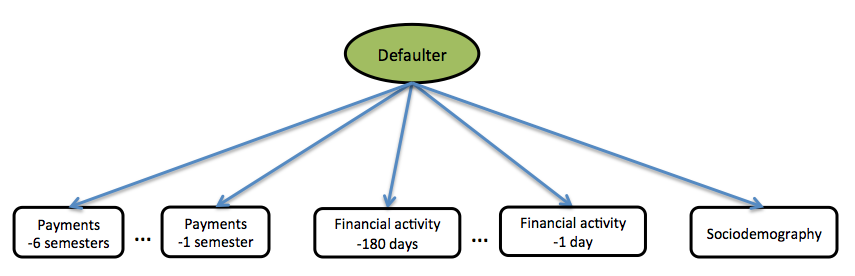
\includegraphics[scale=0.45]{./figures/CajaMarModel0}
\caption{\label{Figure:CajaMarStatic}Global structure of the static model. Each blue box represents a set of variables measures during the same day.
The variables within a box can be connected (e.g. according to a tree structure and, globally, conforming a TAN).}
\label{fig:static}
\end{center}
\end{figure}


%\begin{figure}[ht]
%\begin{center}
%\begin{tikzpicture}[->,>=stealth,shorten >=1pt,auto,node distance=2cm,semithick,
%        amarillo/.style={fill=yellow,rectangle,draw},
%        rojo/.style={fill=red,rectangle,draw,rounded corners}]
%        \node[green] (default) {Default};
%        \node (dot) [below of=default] {$\cdots$};
%        \node[amarillo] (tran1) [left of=dot] {Day -180};
%        \node[amarillo] (tran180) [right of=dot] {Day -1};
%        \draw (default) to (tran1);
%        \draw (default) to (tran180);
%\end{tikzpicture}
%\end{center}
%\caption{\label{Figure:CajaMarStatic}Global structure of the static model. Each yellow box represents a set of variables measures during the same day.
%The variables within a box can be connected (according to a tree structure and, globally, conforming a TAN).}
%\label{fig:static}
%\end{figure}
%---------------------------------------------------------------------------------------------


\begin{figure}
\begin{center}
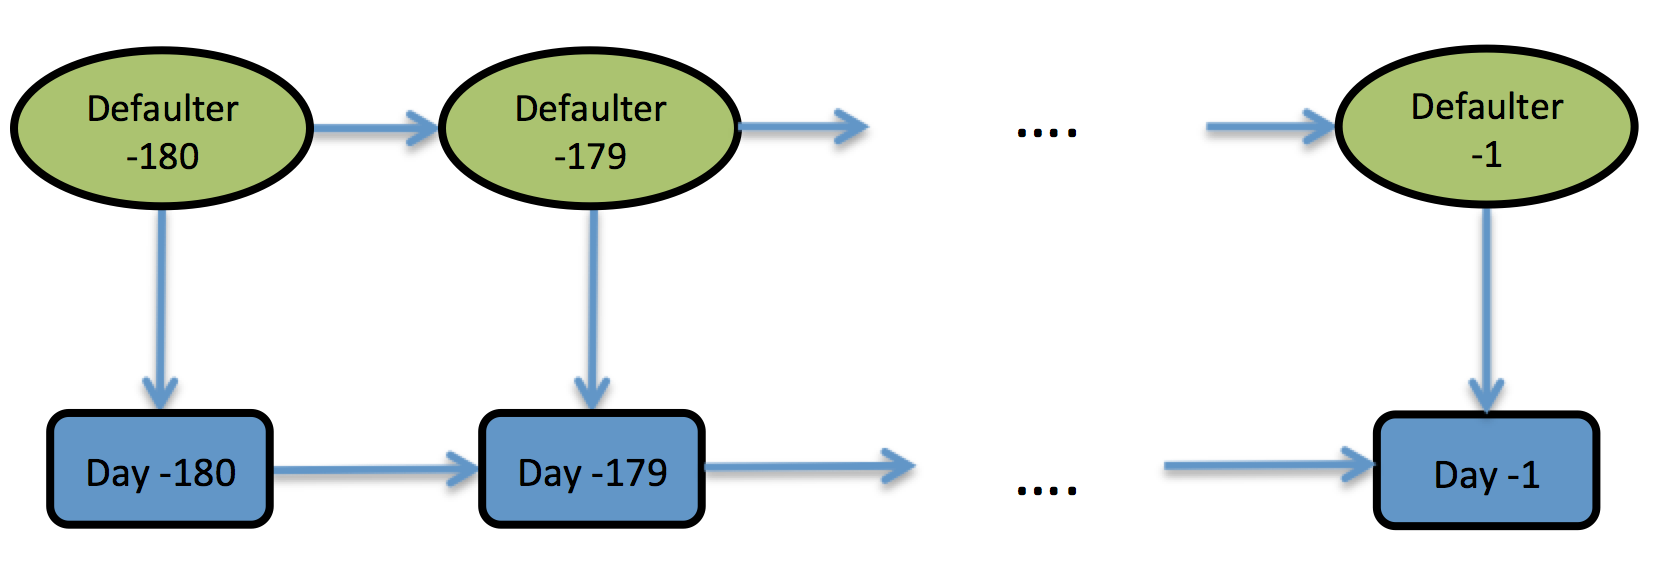
\includegraphics[scale=0.45]{./figures/CajaMarModel1}
\caption{Global structure of the dynamic model. Each yellow box represents a set of variables measures during the same day.
The variables within a box can be connected (according to a tree structure and, globally, conforming a TAN) as well as variables between two consecutive days. Red box refer to the possibility that 
client is defaulter and are temporal connected.}
\label{fig:global_temp}
\end{center}
\end{figure}

%\begin{figure}[ht]
%\begin{center}
%\begin{tikzpicture}[->,>=stealth,shorten >=1pt,auto,node distance=3cm,semithick,
%        amarillo/.style={fill=yellow,rectangle,draw},
%        rojo/.style={fill=red,rectangle,draw,rounded corners}]
%        \node[rojo] (default1) {Default -180};
%        \node[amarillo] (tran1) [below of=default1] {Day -180};
%        \node[rojo] (default2) [right of=default1] {Default -179};
%        \node[amarillo] (tran2) [below of=default2] {Day -179};
%        \node (dot) [right of=tran2] {$\cdots$};
%        \node (blank) [above of=dot] {$~~$};
%        \node[amarillo] (tran180) [right of=dot] {Day -1};
%        \node[rojo] (default180) [above of=tran180] {Default -1};
%        \draw (default1) to (tran1);
%        \draw (default2) to (tran2);
%        \draw (default180) to (tran180);
%        \draw (default1) to [bend left=45] (default2);
%        \draw (default2) to [bend left=45] (blank);
%        \draw (blank) to [bend left=45] (default180);
%        \draw (tran1) to [bend right=45] (tran2);
%        \draw (tran2) to [bend right=45] (dot);
%        \draw (dot) to [bend right=45] (tran180);
%\end{tikzpicture}
%\end{center}
%\caption{Global structure of the dynamic model. Each yellow box represents a set of variables measures during the same day.
%The variables within a box can be connected (according to a tree structure and, globally, conforming a TAN) as well as variables between two consecutive days. Red box refer to the possibility that 
%client is defaulter and are temporal connected.}
%\label{fig:global_temp}
%\end{figure}
%---------------------------------------------------------------------------------------------


%---------------------------------------------------------------------------------------------
\subsubsection*{Dynamic Model} 

In this approach we will consider the the dynamic structure of the problem. These dynamics are present because the behaviour of the customers evolves over time (e.g. the account balance is continuously changing from month to another, the level of incomes, etc.)  as well as the labelling as defaulter or non-defaulter customer (e.g. one customer can be creditworthy and, but after some time, be in bankrupt for becoming unemployed). 


\begin{figure}
\begin{center}
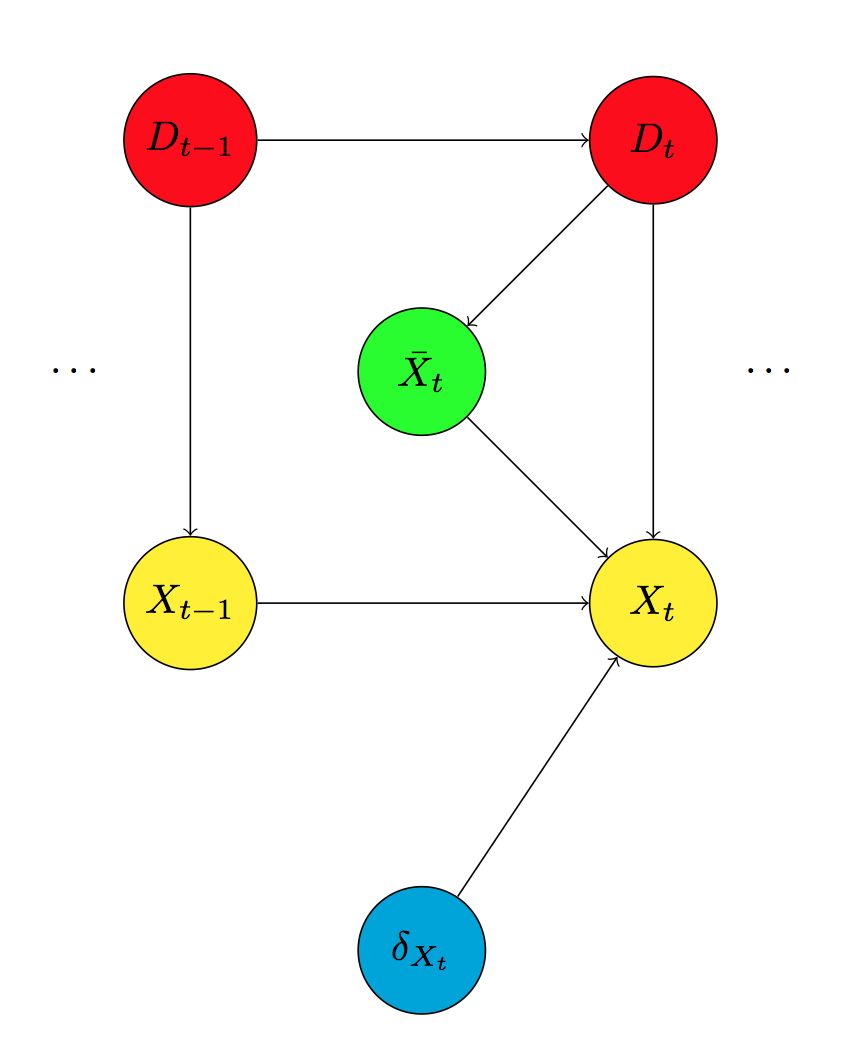
\includegraphics[scale=0.35]{./figures/CajaMarModel2}
\caption{Basic component of the structure of the dynamic model.}
\label{fig:component}
\end{center}
\end{figure}

%\begin{figure}[ht]
%\begin{center}
%\begin{tikzpicture}
%  \node[circle,fill=yellow,draw, minimum size=1.1cm] (Xt1) at (1,1) {$X_{t-1}$};
%  \node[circle,fill=yellow,draw, minimum size=1.1cm] (Xt) at (5,1) {$X_t$};
%  \node[circle,fill=green,draw, minimum size=1.1cm] (avg) at (3,3) {$\bar{X}_t$};
%  \node[circle,fill=cyan,draw, minimum size=1.1cm] (ind) at (3,-2) {$\delta_{X_t}$};
%  \node[circle,fill=red,draw, minimum size=1.1cm] (D) at (5,5) {$D_t$};
%  \node[circle,fill=red,draw, minimum size=1.1cm] (Dt1) at (1,5) {$D_{t-1}$};
%  
%  \node at (0,3) {$\cdots$};
%  \node at (6,3) {$\cdots$};
%  
%  \draw[->] (Dt1) to (Xt1);
%  \draw[->] (Dt1) to (D);
%  \draw[->] (D) to (Xt);
%  \draw[->] (D) to (avg);
%  \draw[->] (Xt1) to (Xt);
%  \draw[->] (avg) to (Xt);
%  \draw[->] (ind) to (Xt);
%  
%  
%  
%\end{tikzpicture}
%\end{center}
%\caption{Basic component of the structure of the dynamic model.}
%\label{fig:component}
%\end{figure}

Figure~\ref{fig:global_temp} represents the global idea of the temporal model. It can be compactly
represented by a dynamic Bayesian network made of components as the one displayed in 
Figure~\ref{fig:component}. $D_t$ represents the class variable at time slice $t$ (i.e. defaulting or non-defaulting client). Each feature
variable at time $t$, denoted as $X_t$, is linked to the same variable at time $t_1$: $X_{t-1}$
as well as to a \emph{memory variable} $\bar{X}_t$ that represents the average value of $X$
during the last $180$ time slices (days). Finally, an indicator variable $\delta_{X_t}$ may
be included if the variable is such that is observed many times at point 0. This is the case as,
for instance, payments by credit card, where many of the days can be equal to zero for most of
the customers.


The process of building this static model would consist of the following steps:

\begin{itemize}
\item Construct \emph{1 table} for each day.
\item Build a \emph{dynamic} BN classifier (NB or TAN like structure extended in a dynamic fashion). 
\item Update risk profiles using the classifier.
\end{itemize}





%\subsubsection*{Model Structure}
%
%From a probabilistic modelling point of view, Caja-Mar faces two different problems [][]: the prediction of the risk of defaulting of a customer in the next two years; and the extraction of profiles of ``desirable'' prospective customers. 
%
%The risk prediction problem has been modelled as supervised dynamic prediction problem.  We are given a data base with a set of variables or predictors (some of them manually built by CajaMar's experts) describing the financial behaviour of the customers and, also, whether the customer is considered as defaulter and non defaulter according to CajaMar standards (i.e. a binary class variable). The dynamic component of the problem needs to be considered because the behaviour of the customers evolves over time (e.g. the account balance is continuously changing from month to another, the level of incomes, etc.)  as well as the labelling as defaulter or non-defaulter customer (e.g. one customer can be creditworthy and, but after some time, be in bankrupt for becoming unemployed). More specifically, the proposed model is expected to answer the following question: which is the probability that this customer will  default in some of his/her loans in two years? And this prediction has to be made only using the customer's behavior in the last 180 days \footnote{This limit is imposed by the Bank of Spain.}.
%
%The graphical structure of the dynamic probabilistic graphical model devised for this problem is given in Figure \ref{Figure:CajaMarModel1}.  The yellow square boxes ``Day -180'', ..., ``Day-1'' represents the temporal evolution of the predictor variables. The model only refers to 180 days because this is the imposed limit of days when making predictions. Similarly, the class variable ``default'' is assumed to evolve over time but with the relevant different that the default class sequence refers to a point in the time \textbf{two years later} than  the point in the time the daily predictor variables. 



\subsubsection*{Data Analysis}

